\begin{Q}
\textbf{Pretrained VLM Adaptation for Visual Question Answering. 50 Points}

In this problem, you will use a pretrained visual-language model (VLM) for a small synthetic visual question answering task.
The lecture notebook uses a Hugging Face processor and multimodal prompting, and this homework follows the same general pattern.
Unlike the earlier frozen-feature version, here the VLM directly sees the image and the text prompt.
Your job is to implement zero-shot VLM inference and LoRA fine-tuning.

The visible files are
\[
\texttt{data/train.jsonl},\quad
\texttt{data/val.jsonl}.
\]
Each row points to a rendered image file under \texttt{data/images/...}.
Students should run the script only in \texttt{--mode train} locally.
Gradescope will run hidden \texttt{data/test.jsonl} rows with hidden test images.

You are provided with a starter Python file.
Your task is to fill in \emph{only} the functions whose docstring begins with \textbf{Implement:}.
For clarity, the main graded functions in this assignment are:
\begin{align*}
&\texttt{build\_prompt},\ 
\texttt{build\_model\_and\_processor},\\
&\texttt{predict\_zero\_shot},\ 
\texttt{train\_lora\_adapter}.
\end{align*}

\medskip
\noindent\textbf{Data format.}
Each JSON line stores:
\begin{itemize}
\item the deterministic scene specification,
\item the image path,
\item the question,
\item the answer.
\end{itemize}

\begin{center}
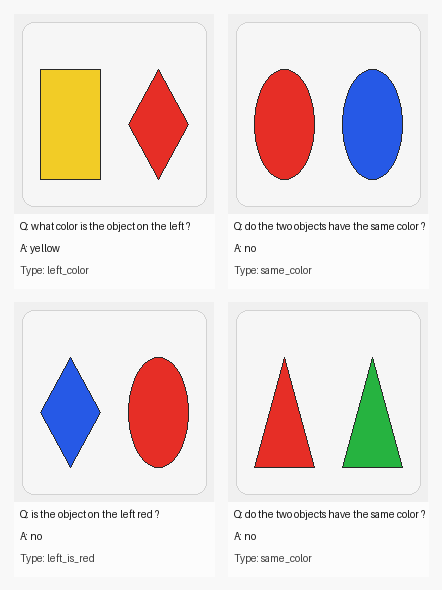
\includegraphics[width=0.72\linewidth]{figures/vlm_train_examples.png}

\small Representative training examples for the VLM problem, showing the rendered image together with its question and answer.
\end{center}

\medskip
\noindent\textbf{VLM pipeline.}
The released code uses the pretrained model \texttt{HuggingFaceTB/SmolVLM-500M-Instruct}.
For each example:
\begin{itemize}
\item the processor receives the image and the prompt together,
\item the processor converts the image into model-specific visual inputs,
\item the processor tokenizes the prompt text,
\item the VLM consumes both modalities together and predicts the answer.
\end{itemize}
The fixed instruction is:
\[
\texttt{Answer with one word only from: red, blue, green, yellow, yes, no.}
\]
For a question such as ``what color is the object on the left ?'', the user-side prompt is:
{\small
\texttt{<image> Answer with one word only from: red, blue, green, yellow, yes, no.}\\
\texttt{Question: what color is the object on the left ?}
}
In the released configuration, the processor uses \texttt{do\_image\_splitting=False}, a longest-edge image size of 256, and \texttt{image\_seq\_len=16}, so the \texttt{<image>} portion corresponds to 16 visual tokens.

\medskip
\noindent\textbf{What Is Frozen And What Is Trained?}
Zero-shot evaluation runs the pretrained VLM directly with no updates.
During training, you should keep the base VLM and attach a LoRA adapter, then optimize only the LoRA parameters on the visible training split.
So the model remains the same pretrained VLM throughout both zero-shot evaluation and fine-tuning.

\begin{center}
  \scalebox{0.8}{
\begin{tikzpicture}[
  node distance=0.8cm and 0.9cm,
  box/.style={draw, rounded corners, align=center, minimum height=1.0cm, minimum width=2.45cm, fill=gray!8},
  frozen/.style={box, fill=blue!8},
  trainable/.style={box, fill=red!8},
  arr/.style={-{Latex[length=2.2mm]}, thick}
]
\node[frozen] (img) {image};
\node[frozen, right=of img] (proc) {processor};
\node[frozen, below=of proc] (text) {prompt text};
\node[frozen, right=of proc] (vlm) {pretrained VLM\\SmolVLM-500M};
\node[trainable, right=of vlm] (lora) {LoRA adapter};
\node[trainable, above=of lora] (ans) {answer token};

\draw[arr] (img) -- (proc);
\draw[arr] (text) -- (proc);
\draw[arr] (proc) -- (vlm);
\draw[arr] (vlm) -- (lora);
\draw[arr] (lora) -- (ans);
\end{tikzpicture}
}

\small The processor converts the image and prompt into the inputs expected by the pretrained VLM. Zero-shot uses the pretrained VLM directly, while fine-tuning updates only the LoRA adapter.
\end{center}

\medskip
\noindent\textbf{Training protocol.}
The script:
\begin{itemize}
\item runs zero-shot VLM inference on the validation split,
\item fine-tunes the VLM with LoRA on the full visible training split,
\item reports train loss, validation loss, and validation accuracy after each epoch,
\item saves \texttt{outputs/vlm\_model.pt},
\item saves a small labeled example sheet with image, question, and answer,
\item later evaluates the saved checkpoint on hidden test data.
\end{itemize}

\medskip
\noindent\textbf{Autograder.}
Gradescope will:
\begin{itemize}
\item run unit tests on the four core functions above,
\item run your training script,
\item load \texttt{outputs/vlm\_model.pt},
\item evaluate the submitted checkpoint on hidden test data.
\end{itemize}
The score breakdown is:
\begin{itemize}
\item 40 points for correct implementations of the four core functions,
\item 10 points for reporting the requested validation numbers from \texttt{--mode train} and submitting a checkpoint that is evaluated on hidden test data.
\end{itemize}

\begin{enumerate}

\item \textbf{\texttt{build\_prompt}: construct the VLM prompt (10 points).}
Implement \texttt{build\_prompt(question)}.
It should return the plain text prompt used together with the image in the processor call.

\item \textbf{\texttt{build\_model\_and\_processor}: load the pretrained VLM (10 points).}
Implement \texttt{build\_model\_and\_processor(model\_name, device)}.
It should load the Hugging Face processor and the pretrained VLM, disable image splitting for a lighter visual path, move the model to the target device, and return both objects.

\item \textbf{\texttt{predict\_zero\_shot}: run zero-shot VLM inference (10 points).}
Implement \texttt{predict\_zero\_shot(model, processor, row, data\_dir, device)}.
It should build the multimodal prompt, run \texttt{model.generate(...)}, decode the generated continuation, and return one answer string.

\item \textbf{\texttt{train\_lora\_adapter}: fine-tune the pretrained VLM with LoRA (10 points).}
Implement the training loop with:
\begin{itemize}
\item LoRA attachment to the pretrained VLM,
\item AdamW,
\item validation after each epoch,
\item best-model selection by validation loss (tie-break by validation accuracy),
\item restoration of the best checkpoint before returning.
\end{itemize}

\item \textbf{Training-Mode Report and Checkpoint Submission (10 points).}
Run the script in \texttt{--mode train} and report:
\begin{itemize}
\item the zero-shot validation loss and accuracy,
\item the train loss, validation loss, and validation accuracy after each epoch,
\item the final \texttt{final-train} validation result from the saved checkpoint.
\end{itemize}
Students do not have access to the hidden test split. Submit \texttt{outputs/vlm\_model.pt} to Gradescope, and the autograder will evaluate it on hidden test data.

\begin{solution}

  \begin{tabular}{lcccc}
\hline
Method & Config & Train loss & Val loss & Val acc \\
\hline
Zero-shot VLM & -- & -- & 0.8750 & 0.1250 \\
LoRA VLM & epoch-1 & 4.3336 & 1.9859 & 0.5625 \\
LoRA VLM & epoch-2 & 1.1559 & 0.7250 & 0.8250 \\
LoRA VLM & epoch-3 & 0.3642 & 0.3019 & 0.8625 \\
LoRA VLM & final-train & 0.3642 & 0.3019 & 0.8625 \\
\hline
\end{tabular}

on test data, grade is acc/base-accuracy truncated at 1, where base-accuracy is 0.91 below


test-final-train: loss=0.2680 acc=0.9125

\end{solution}

\end{enumerate}
\end{Q}
